\chapter{Technical Approach}

\section{System Requirements}

\begin{enumerate}
\item Ubuntu 14.04
\item HHVM 3.10.0
\item Java Runtime Environment 1.7
\end{enumerate}

\section{HHVM Bytecode Processing}
HHVM compiles Hack and PHP into an intermediate bytecode. The intermediate bytecode is processed to build control flow graphs.

\subsection{Intra-Procedural Control Flow Graph Construction}
Control Flow Graph (CFG) is a graph representation of a program that represents all the paths that might be traversed through during its execution, which is the basis for performing variable liveness check and building def-use/use-def chains. The procedure for building a CFG has been extensively investigated and there is a standard algorithm for building CFG from intermediate representations (Hip-Hop byte code, in this case):

\subsubsection{Basic Block Partitioning}
Identify leader statements (i.e. the first statements of basic blocks) by using the following rules:

\begin{enumerate}
\item Identify leader statements
\begin{enumerate}
\item The first statement is a leader
\item Any statement that is the target of a branch statement is a leader (for most intermediate languages these are statements with an associated label)
\item  Any statement that immediately follows a branch or return statement is a leader
\end{enumerate}
\item The basic block corresponding to a leader consists of the leader, plus all statements up to but not including the next leader or up to the end of the program
\end{enumerate}

\subsubsection{Control Flow Graph Construction}
The basic block corresponding to a leader consists of the leader, plus all statements up to but not including the next leader or up to the end of the program
\begin{enumerate}
\item There is a branch from the last statement of B1 to the first statement of B2, or
\item Control flow can fall through from B1 to B2 because
\begin{enumerate}
\item B2 immediately follows B1, and
\item B1 does not end with an unconditional branch
\end{enumerate}
\end{enumerate}

\subsection{Data Flow Analysis}
In order to keep track of how each variable is used in the program, it is critical to perform data flow analysis, which outputs def-use chains and use-def chains, both of which are critical to the later stages of the project.
\subsubsection{Def-Use Chains and Liveness Analysis}
Def-use chain is used to keep information about reaching definition of a variable. Specifically, for each use of a variable x, its def-use chain is a list of the definitions of x reaching that use. Liveness Analysis is used to get def-use chains.
\begin{itemize}
\item At each program point:
\begin{itemize}
\item Which variables contain values computed earlier and needed later – they are said to be live
\end{itemize}

\item For instruction I:
\begin{itemize}
\item in[I]: live variables at program point before I
\item out[i]: live variables at program point after I
\end{itemize}

\item For a basic block B:
\begin{itemize}
\item in[B]: live variables at beginning of B
\item out[B]: live variables at end of B
\end{itemize}

\item DU[I] = out[I] – in[I]
\item Note:
\begin{itemize}
\item in[I] = in[B] for first instruction of B
\item out[I] = out[B] for last instruction of B
\end{itemize}

\end{itemize}

\algdef{SE}[UNTIL]{Until}{EndUntil}[1]{\algorithmicuntil\ #1\ \algorithmicrepeat}{\algorithmicend\ \algorithmicuntil}%
\begin{algorithm}
\caption{Liveness Calculation in CFG}
\begin{algorithmic}
\For{Each instruction $I$}
	\State{in[I] $\gets$ $\emptyset$}
	\State{out[I] $\gets$ $\emptyset$}
\EndFor
\Until{no change in set}
	\For{Each instruction $I$}
		\State{in[I] $\gets$ (out[I] - def[I]) $\cup$ use[I]}
	\EndFor
	\For{Each basic block $B$}
		\State{out[B] $\gets$ $\cup$ in[S] (S $\in$ Successor[B])}
	\EndFor
\EndUntil
\end{algorithmic}
\end{algorithm}

\subsubsection{Use-Def Chains and Reaching-definition Analysis}
To the opposite of def-use chains, use-def chain is used to keep track of reachable definitions for a use of a variable. Reaching-definition analysis is the method to get use-def chains.
\begin{itemize}
\item For instruction I:
\begin{itemize}
\item in[I]: reaching definitions going into I
\item in[I]: reaching definitions going into I
\item in[I]: reaching definitions going into I
\item kill[I]: definition at I
\end{itemize}
\item For a basic block B:
\begin{itemize}
\item in[B]: reaching definitions going into B
\item out[B]: reaching definitions coming out of B
\end{itemize}
\item UD[I] = in[I] – out[I]
\end{itemize}

\begin{algorithm}
\caption{Reaching-def Calculation in CFG}
\begin{algorithmic}
\For{Each instruction $I$}
	\State{in[I] $\gets$ $\emptyset$}
	\State{out[I] $\gets$ $\emptyset$}
\EndFor
\Until{no change in set}
	\For{Each instruction $I$}
		\State{out[I] $\gets$ (in[I] - kill[I]) $\cup$ gen[I]}
	\EndFor
	\For{Each basic block $B$}
		\State{in[B] $\gets$ $\cup$ out[P] (P $\in$ Predecessor[B])}
	\EndFor
\EndUntil
\end{algorithmic}
\end{algorithm}

\section{String Automaton Construction}
The second step is to construct estimated input variables by using the result of data flow analysis. The Use-Def chain is particularly useful, because it allows a used variable to be traced back to where it is originally defined.

As string typed inputs are the most common interface inputs of PHP web applications, this section mainly focuses on string estimation. Christensen, Møller, and Schwartzbach \cite{ref4} have proposed a promising algorithm for performing regular expression estimation for a string variable through data flow analysis. In this section a third-party package, dk.brics.automaton, is used. dk.brics.automaton is an open-source Java package implemented based on the research of Christensen, et al. It is language-independent, and supports most commonly used string operations. dk.brics.automaton is able to take flow graph composed of operators and operands (known characters), and generate a definite finite automaton (DFA), which is an estimated regular expression for the analyzed string.

In order to build a complete flow-graph for a string variable, a stack is used to mimic HHVM executions. During HHVM execution, variables and functions are pushed to top of a running stack. Each action (arithmetic operations, string operations, etc.) takes one or more elements popped from the stack, and pushes the new result to stack top. Sometimes when multiple operations are chained together, the stack actions will have a hierarchical form. For example, the stack action for d = (a + b + c) is:

\begin{forest}
  [Set% root
    [var d]
    [Plus% root of \section{•}
      [var c]
      [Plus
        [var b]
        [Get
          [var a]
        ]
      ]
    ]
  ]
\end{forest}

\begin{table}
\begin{tabular}{c}
Supported PHP String Operations \\
\hline
Concat \\
StrComp \\
Substr \\
ToUpperCase \\
ToLowerCase \\
Reverse \\
Trim \\
Split \\
Replace \\
StrToTime \\
\label{Supported PHP string operations}
\end{tabular}
\end{table}

\section{Interface Discovery and Grouping}

In this step, variables exposed by the application interface(input variables) are identified and grouped logically. This part of the program implements two interface discovery algorithms proposed by Halfond and Orso \cite{ref3}.


% % This is a figure in landscape orientation
% \begin{sidewaysfigure}
% 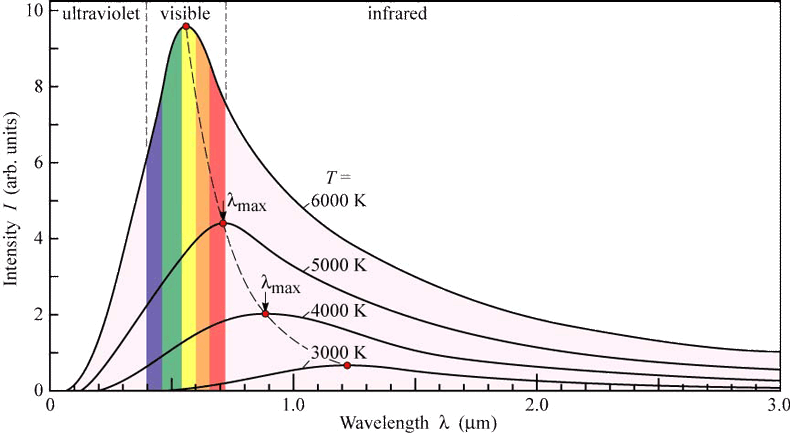
\includegraphics[width=\textwidth]{figures/exampleFigure.png}
% \caption{This is another example Figure, rotated to landscape orientation.}
% \label{LandscapeFigure}
% \end{sidewaysfigure}
